%.-------------------------------------------------------------------------------------------------------------------------------------------------------------
\subsection{Back-end}
\subsubsection{Package diagram}
The Java code has a Javadoc which can be accesssed in \href{https://github.com/pm390/MaldiniPaone/tree/master/Implementation\&Testing/SafeStreets/doc}{our github repository} 
Here we present the overall structure of the project at different levels.
\begin{figure}[h]
\centering
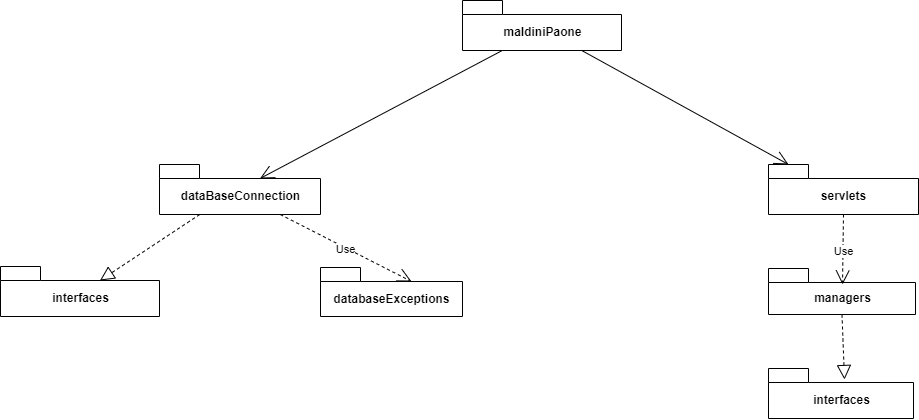
\includegraphics[width=\textwidth]{Images/packageDiagram.png}
\caption{\label{fig:pK} Package diagram of the main packages}
\end{figure}
In this diagram a basic view of the code structure is seen. The source can be divided in mainly two sub-parts. The first part concerning the connection to the database which is handled by the classes in the databaseConnection package and a second part
which communicates with client devices which is handled by the Servlets implemented in the servlet package.
The database Connection package has two sub packages one to define the interfaces it exposes to the other classes, the other with the Exception Classes which can be thrown by the classes in the package.
The servlets package classes communicates with the managers in the managers packkage which provides interfaces to allow access to the needed functionalities.
In this diagram the utilities package and it's sub packages are not shown for the sake of clarity. 
This package contains useful objects, beans and constants which are used through the whole developement.
\clearpage
\subsubsection{ Database Connection}
\begin{figure}[h]
\centering
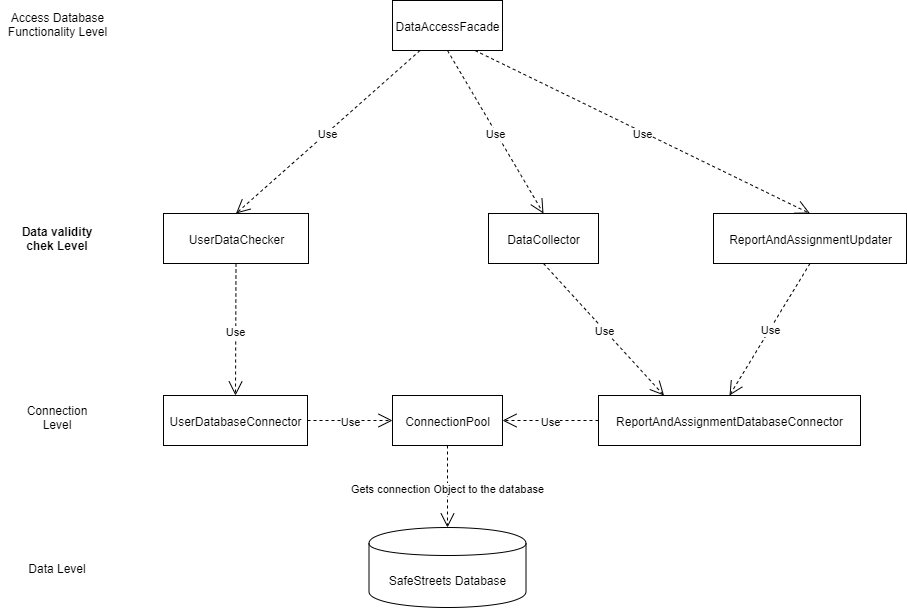
\includegraphics[width=\textwidth]{Images/databaseConnection.png}
\caption{\label{fig:pK} databaseConnection classes}
\end{figure}
This diagram shows the Classes in the databaseConnection package the database is also shown to present which component instantiates connection with it. A clear separation of concerns is shown between the different classes:
\begin{itemize}
\item Connection Level : classes in this level have 2 main functions the instantiation of connection which is done by the ConnectionPool and using the instatiated connections to get data ,save data, update data from the database.
The latter function is implemented in two separated classes to divide the class managing information concerning the user accounts and the one managing information concerning reports and assignments.
Implements the functionalities.
\item Data validity check Level: classes in this level checks that input values for accessing the database are correct. This layer protects the possible accesses to the database with invalid values avoiding the instantiation of useless connection which may slow down the server. This level throws the appropriate exceptions if the database connection couldn't be instantiated on the lower level or if the parameters are invalid.
Controls access to the functionalities.
\item Access Database Functionality Level : this level contains a class DataAccessFacade as the name says it is a facade and so it presents to the other packages the functionalities that the database conneciton package provides. This layer contains almost only call to functions provided by the beneath level to allow a clear separation of the functionalities of the package.
Allows access to the functionalities.
\end{itemize}
\clearpage
\subsubsection{Servlets}
\begin{figure}[h]
\centering
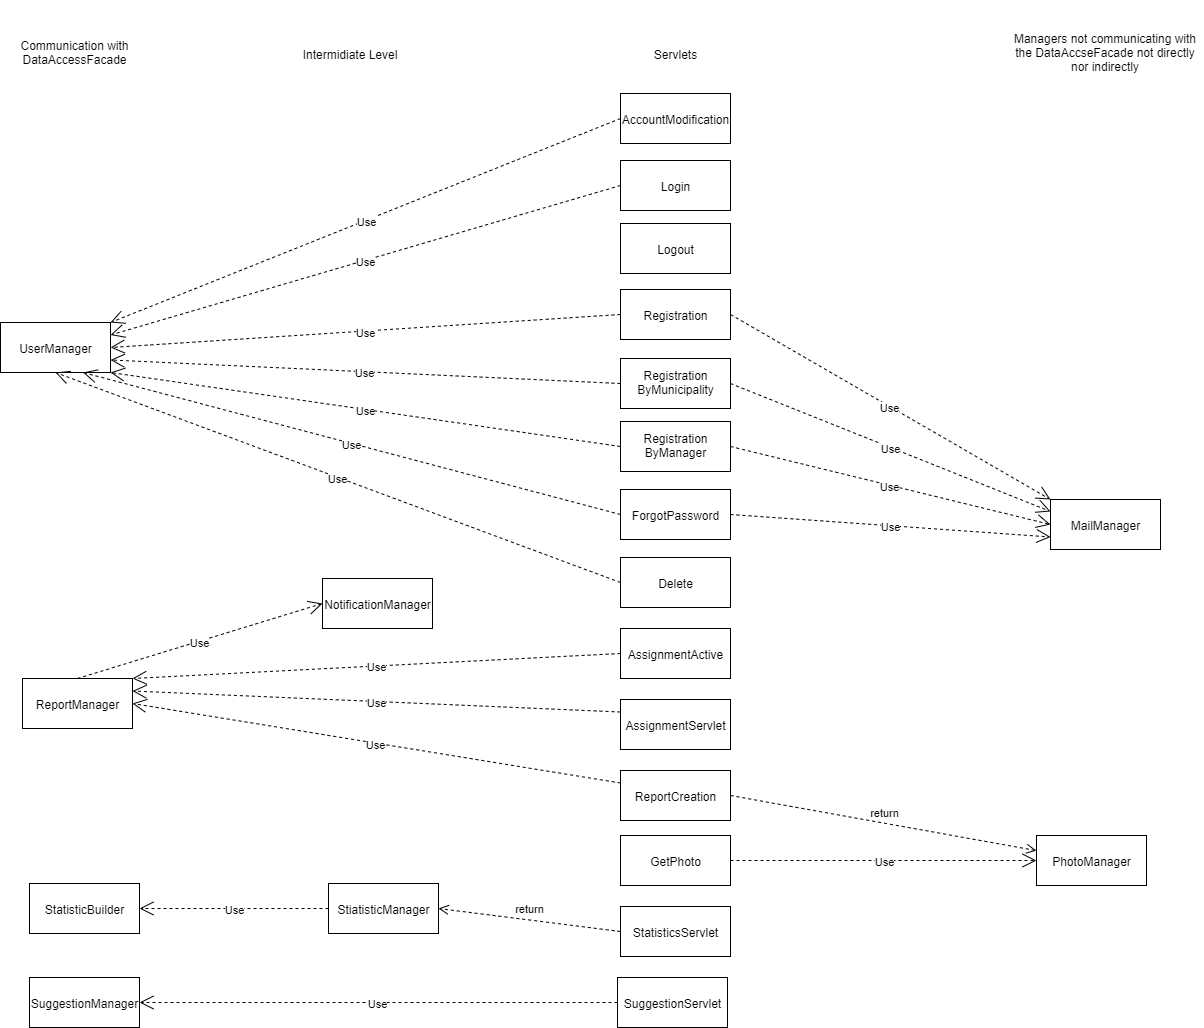
\includegraphics[width=\textwidth]{Images/Servlets.png}
\end{figure}
The Servlet package's classes are shown in the above diagram.
The functionalities provided by the servlets to the end users are provided to the servlets by managers in the package. 
The managers  on the left part communicates with the DataAccess facade to retrieve, save or modify data on the database 
The Intermediate level shown Contains classes which communicates indirectly with the database because informations used by it comes from communications with the database. The servlets provides functionalities of the service to the clients of the web application and of the mobile application.
On the right part of the image 2 managers are shown. Those managers doesn't communicate directly with the database and allows the system to save photos and to send mails to the clients.
\clearpage
\subsection{Front End }
\subsubsection{Web App}
The web application is composed of an html file , a css file developed by us , css files of leaflet to present the map , external javascript imported libraries(jquery, leaflet and openAlpr) and different javascript source files.
The html file contains the single page application which allows municipalities and managers to access their functionalities.
The javascript source files are basicFunctionalities.js and ourMap.js, the first source adds to the page the dinamic behaviour of buttons and avoids synchronous requests to the server using ajax get and post requests, the second source handles the creation of the map and the binding of events to update the map and defines the  behaviour when the user clicks on markers on the map, the other javascript files are used to set up the functionalities of open alpr and use them to recognize license plates in a photo.

